\documentclass[12pt, a4paper]{article}

\usepackage{listings}
\usepackage{color}
\usepackage{enumitem}
\usepackage{amsthm}
\usepackage{amssymb}
\usepackage{listings}
\usepackage{setspace}
\usepackage{graphicx}
\graphicspath{ {./figures/} }


\title{Deep Learning Fundamentals}
\author{William Darko}
\date{Summer 2021}

\pagenumbering{arabic}

\begin{document}

\maketitle
\newpage

\tableofcontents

\newpage

\section{About this course}
\paragraph*{}
Explore deep learning from scratch or broaden understanding of deep learning, via
practical hands-on code examples to solve concrete problems. We'll
utilise the Python language, and deep learning framework Keras with Tensor flow as a backend engine



\newpage

\section{Resources}

\begin{itemize}
   \item \textbf{Deep Learning with Python} (1st Edition) by François Chollet.
   Manning publisher
\end{itemize}

\newpage

\section{What is deep learning?}

\subsection{Artificial Intelligence}
{
   \centering
   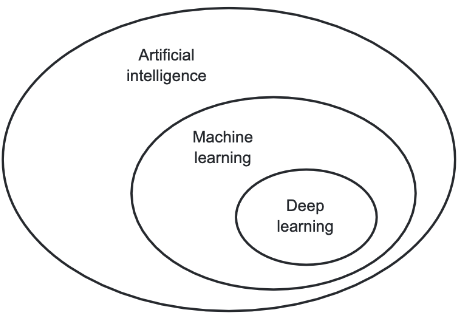
\includegraphics[width=8cm]{AI_Umbrella.png}

   the umbrella of Artificial intelligence

}

\paragraph*{}
We'll define Artificial intelligence to be the \textit{effort to automate intellectual 
tasks normally performed by humans.} AI is the general field that encompasses machine learning,
which deep learning is a subfield of.

\begin{itemize}
   \item Early AI took the approach of programmers manually implementing a large set of 
   rules for manupulating knowledge; this was known as \textbf{symbolic AI}.
   
   \item Symbolic AI turned out intractable, when applied to more complex problems like
   image classification, speech recogition, language translation, etc.
   
   \item Machine Learning was the new AI paradigm that rose to replace symbolic AI. It arises
   from the question: can computers go beyond what we tell it to do? How do computers learn
   on their own how to perform a specific task.
\end{itemize}

{
   \centering
   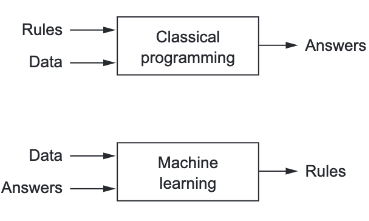
\includegraphics[width=6cm]{ML_new_paradigm.png}

    rules instead of answers in the ML paradigm

}

\begin{itemize}
   \item Recent AI trend driven by increase in computing power (faster hardware), and larger datasets.
\end{itemize}

\subsection{Learning representations from data}

\paragraph*{}
To do basic machine learning, three things are needed:
\begin{enumerate}
   \item \textbf{Input data} such as sound files, images, text documents, etc.
   \item \textbf{Examples of expected output} for training purposes
   \item \textbf{A way to measure the success of the algorithm} to determine the distance between
   algorithm's current output, and exptected output. 
\end{enumerate}

\textbf{The central problem in machine learning, and deep learning is to meaningfully transform data}.
Meaning, to learnin useful representations of the input data, which get us closer to the exptected output.
The learning aspect involves finding data transformations within an already defined set of operations
called the \textbf{hypothesis space}.

\end{document}